%%%%%%%%%%%%%%%%%%%%%%%%%%%%%%%%%%%%%%%%%%%%%%%%%%%%%%%%%%
%%
%% MARK: Title
%%
%%%%%%%%%%%%%%%%%%%%%%%%%%%%%%%%%%%%%%%%%%%%%%%%%%%%%%%%%%

\chapter*{\S B30. Embedding a Diffeological Space \hbox{Into its Powerset}}
\setcounter{footnote}{0}

%%%%%%%%%%%%%%%%%%%%%%%%%%%%%%%%%%%%%%%%%%%%%%%%%%%%%%%%%%
%%
%% MARK: Abstract
%%
%%%%%%%%%%%%%%%%%%%%%%%%%%%%%%%%%%%%%%%%%%%%%%%%%%%%%%%%%%

\begin{abstract}
  In this note we shall see that the natural inclusion of a diffeological space into its powerset is an embedding,
  and a closed embedding if the space is Hausdorff.
\end{abstract}

%%%%%%%%%%%%%%%%%%%%%%%%%%%%%%%%%%%%%%%%%%%%%%%%%%%%%%%%%%
%%
%% MARK: Content
%%
%%%%%%%%%%%%%%%%%%%%%%%%%%%%%%%%%%%%%%%%%%%%%%%%%%%%%%%%%%

The main ingredient is the \emph{powerset diffeology} of a diffeological space,
defined in Exercise 62 of the textbook \cite{PIZ13}.
We recall,
in the first article,
the results of this exercise.

\begin{Article}{The inclusion map.}{}
  Let $X$ be a diffeological space and $\fP(X)$ be its powerset,
  equipped with the powerset diffeology.
  The natural \emph{inclusion map}
  $$%
    j \colon X \to \fP(X) \quad \text{with} \quad j(x) = \{x\},
  $$%
  is smooth and is an induction \cite[\textsection\,1.29]{PIZ13}.
\end{Article}

\begin{proof}
  Let $P: U \to X$ be a plot in $X$.
  We must check that $j \circ P: r \mapsto \{P(r)\}$ is a plot for the powerset diffeology.
  
  For all $r_0 \in U$ and for all plots $Q_0$ with values in $\{P(r_0)\}$,
  which is necessarily constant,
  define the following family of constant plots:
  $$%
    r \mapsto Q_r : \Domain(Q_0) \to X, \quad \text{with} \quad Q_r(s) = P(r).
  $$%
  Since $\Val(Q_r) \subset j(P(r)) = \{P(r)\}$,
  and $(r,s) \mapsto Q_r(s) = P(r)$ is clearly smooth,
  the conditions to be a powerset plot are satisfied by $j \circ P$.
  Thus $j$ is smooth.
  
  Let us check that $j$ is now an induction.
  Let $P: U \to \fP(X)$ be a powerset plot with values in $j(X)$.
  We must check that $j^{-1} \circ P$ is a plot in $X$.
  Indeed,
  for all $r \in U$ there exists $x_r \in X$ such that $P(r) = \{x_r\}$.
  For any fixed $r_0 \in U$ and for any plot $Q_0$ such that $\Val(Q_0) \subset P(r_0) = \{x_{r_0}\}$,
  there exists an open neighborhood $V$ of $r_0$ and a smooth family $r \mapsto Q_r$ of plots,
  defined on $V$,
  such that $\Val(Q_r) \subset P(r) = \{x_r\}$.
  Thus $(s,r) \mapsto Q_r(s) = x_r = j^{-1} \circ P(r)$ is locally smooth,
  and $r \mapsto x_r$ is a plot of $X$.
\end{proof}

\begin{Article}{Embedding $X$ into its powerset.}{}
  The inclusion $j: X \to \fP(X)$ is not just an induction;
  it is an embedding \cite[\textsection\,2.13]{PIZ13}.
  That is,
  the pullback of the D-topology of $\fP(X)$ to $X$ coincides with the D-topology of $X$.
\end{Article}

\begin{proof}
  We must prove that,
  for any D-open subset $\cO \subset X$,
  there exists a D-open set $\cO'$ in $\fP(X)$ such that $j(\cO) = j(X) \cap \cO'$.
  
  Define
  $$%
    \cO' = \{ A \in \fP(X) \mid A \cap \cO \neq \varnothing \}.
  $$%
  Clearly $j(\cO) = j(X) \cap \cO'$. It remains to prove that $\cO'$ is D-open in $\fP(X)$.
  %
  For any plot $P: U \to \fP(X)$,
  we must show that
  $$%
    P^{-1}(\cO') = \{ r \in U \mid P(r) \cap \cO \neq \varnothing \}
  $$%
  is open.
  %
  Let $r_0 \in P^{-1}(\cO')$,
  so $P(r_0) \cap \cO \neq \varnothing$.
  Pick $x_0 \in P(r_0) \cap \cO$ and the constant plot $Q_0(s) = x_0$.
  By the definition of the powerset diffeology,
  there exists a smooth family of plots $Q_r$ for $r$ near $r_0$ such that $\Val(Q_r) \subset P(r)$ and $(s,r) \mapsto Q_r(s)$ is smooth.
  %
  Since $\cO$ is open,
  by continuity of $Q_r(s)$,
  there exists a product of balls $\Omega = B(s_0, \varepsilon) \times B(r_0, \eta)$ (for some chosen $s_0$) such that for all $(s,r) \in \Omega$, $Q_r(s) \in \cO$.
  The condition $\Val(Q_r) \subset P(r)$ then implies that $P(r) \cap \cO \neq \varnothing$.
  Thus $B(r_0, \eta) \subset P^{-1}(\cO')$,
  so $P^{-1}(\cO')$ is open.
  Therefore $\cO'$ is D-open.
\end{proof}

\begin{Article}{The case of the empty set.}{}
  Let $\fP(X)^\star$ be the subset of non-empty subsets of $X$:
  $$%
    \fP(X)^\star = \fP(X) \setminus \bigl\{ \{\varnothing\} \bigr\}.
  $$%
  Then,
  equipped with the powerset diffeology,
  $\fP(X)$ is the vague adjunction of the singleton $\{\varnothing\}$ to $\fP(X)^\star$,
  as defined in the previous note ``Vague Adjunction of a Point to a Space''.
  This implies in particular that,
  for the D-topology,
  $\{\varnothing\} \subset \fP(X)$ is closed,
  and $\fP(X)$ is the only neighborhood of $\{\varnothing\}$.
\end{Article}

\begin{proof}
  Indeed,
  for a parametrization $P$ in $\fP(X)$ and a point $r_0 \in \Domain(P)$,
  if $P(r_0) = \{\varnothing\}$ then the condition of the powerset diffeology is vacuous.
\end{proof}

\begin{Article}{$X$ in $\fP(X)$.}{}
  If $X$ is Hausdorff for the D-topology,
  then its image $j(X)$ in $\fP(X)^\star$ is closed.
  Equivalently, $j(X) \cup \{\varnothing\}$ is closed in $\fP(X)$.
\end{Article}

\begin{proof}
  Let us show that $\fP(X)^\star \setminus j(X)$ is open.
  Note that
  $$%
    \fP(X)^\star \setminus j(X) = \bigl\{ A \subset X \mid \exists x, y \in A,\ x \neq y \bigr\}.
  $$%
  
  Consider a plot $P: U \to \fP(X)^\star$, and $r_0 \in P^{-1}(\fP(X)^\star \setminus j(X))$.
  Suppose $\{x_0, y_0\} \subset P(r_0)$ with $x_0 \neq y_0$.
  Let $Q_0$ and $Q_0'$ be two constant plots such that
  $\Val(Q_0) = \{x_0\}$ and $\Val(Q_0') = \{y_0\}$.
  By the definition of the powerset diffeology,
  there exist two smooth families $r \mapsto Q_r$ (for $r$ in a neighborhood $V$ of $r_0$)
  and $r \mapsto Q_r'$ (for $r$ in a neighborhood $V'$ of $r_0$)
  such that $\Val(Q_r) \subset P(r)$ and $\Val(Q_r') \subset P(r)$.
  
  Since $X$ is Hausdorff,
  we may choose two disjoint D-open neighborhoods $\cO$ and $\cO'$ of $x_0$ and $y_0$ respectively.
  Given $s_0$ in a common domain of $Q_r$ and $Q_r'$,
  the intersection of the preimages of $\cO$ and $\cO'$ by the continuous maps
  $(r,s) \mapsto Q_r(s)$ and $(r,s) \mapsto Q_r'(s)$ defines an open neighborhood $W \times S$ of $(r_0, s_0)$,
  with $W \subset V \cap V'$,
  such that $Q_r(s) \in \cO$ and $Q_r'(s) \in \cO'$ for all $(r,s) \in W \times S$.
  
  Since $\Val(Q_r) \subset P(r)$ and $\Val(Q_r') \subset P(r)$,
  the condition $\cO \cap \cO' = \varnothing$ ensures that $P(r)$ contains at least two distinct points of $X$ for all $r \in W$.
  Hence $W \subset P^{-1}(\fP(X)^\star \setminus j(X))$.
  
  Thus $P^{-1}(\fP(X)^\star \setminus j(X))$ is open,
  as a union of open subsets.
  Therefore $\fP(X)^\star \setminus j(X)$ is D-open,
  and $j(X)$ is closed in $\fP(X)^\star$.
\end{proof}

\vfill
\centerline{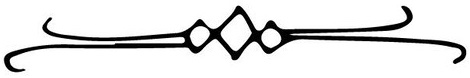
\includegraphics[width=.6\textwidth]{Figures/separator.jpg}}
\vfill
